\chapter{Improving searches for GW associated with GRBs} % Write in your own chapter title
\label{Chapter Five}
%\lhead{Chapter~\ref{ChapterLabel}
% \emph{Improving searches for GW associated with GRBs}} % Write in your own chapter title to set the page header
\section{Introduction}

The sensitivity of triggered searches for gravitational wave inspiral signals associated with short gamma-ray bursts may always be improved by implementing new data analysis techniques that increase the confidence of a possible detection; also, better knowledge of the source itself (astrophysical priors) may restrict the parameter space, making the analysis more sensitive and time and computing--efficient. In this chapter we describe such improvements for both the coincident and the coherent analysis methods: a better estimation of the background data using timeslides for a GW--GRB search and a proposed prior on the inclination angle of the binary.

Short hard gamma-ray bursts are cosmological events and are, on average, closer in luminosity distance than long gamma-ray bursts (see Chapter \ref{Chapter Two}), but those detected with the smallest measured redshifts are still beyond the inspiral range of present day GW detectors; however, this does not exclude the possibility of a future detection of a short burst with a much smaller redshift. Using a trigger from a GRB satellite and performing a GW search around this trigger is just the first step towards making a GW detection (see Chapter \ref{Chapter Four} for two examples of such searches); the second, and equally important part, is, in the case of finding an outstanding GW candidate associated with the GRB trigger, how confident we are that this candidate is indeed a gravitational wave and not arising from detector noise. 

Suppose we have this scenario: a short GRB is detected by a satellite and there is no afterglow that can identify a host galaxy, hence no information of its redshift or luminosity distance (see Chapter \ref{Chapter Two} for an explanation of short GRB afterglow detections). After performing a GW--GRB search one finds a loud (high--SNR) candidate associated with the GRB. The question arises: what is the false alarm probability that we should quote in order for us to claim a GW detection, with no supporting astrophysical information on the distance to the GRB in question? By ``false alarm probability'' we denote the probability that the newly found GW trigger \emph{is} produced by detector noise. This quantity is estimated purely from the statistical properties of the GW stretch of data that we analyzed and is a number we quote at the end of the analysis (see Chapter \ref{Chapter Four} for two such results). We will have to compare this number to an astrophysical quantity that gives information on the GRB. Such an astrophysical quantity would be the probability that the GRB was located at a luminosity distance within the GW detectors' range, and may be estimated from the collective properties of a population of short GRBs for which we know the distances. We describe two ways of estimating this probability.

We will look at a \emph{very} naive model for which we assume a constant number density for short GRBs within a physical spherical volume with a fixed radius of 2 Gpc ($z \approx 0.5$), in other words we consider that short GRBs occur only at very low redshifts. The 2 Gpc limit is chosen so the Euclidean and cosmological volumes are approximately equal. Assuming an optimistic average initial LIGO/Virgo horizon range of 20 Mpc for an ideally located and oriented NS--NS binary, we can express the probability that a certain given burst occurred within the detection volume for the GW detector:

\begin{equation}
\mathrm{P} = \frac{4\pi}{3}\frac{\mathrm{d}N_\mathrm{observable}(\mathrm{V_{detector}}=8 \times 10^{-6} ~\mathrm{Gpc}^3)}{\mathrm{d}N(\mathrm{V_{uniform}}= 8 ~\mathrm{Gpc}^3)} \approx 4 \times 10^{-6}
\label{grb_p}
\end{equation}

This is a very simplified way of estimating the chance that a GRB was within the GW detectors' range: short bursts are not proven to be uniformly distributed in volume (simply because we have not yet detected a very near--by one and the numbers of those with unambiguously determined redshifts are too small to derive any volume distribution); the GW detection range is not constant and depends on a series of parameters (binary localization and inclination, noise PSD etc., see Chapter \ref{Chapter Three} for reference); short bursts are not within redshift $z \approx 0.5$ only. Despite all this, the formula above gives a rough measure of this chance probability, estimated 1 in a million FAP.

A lower bound for the rate of observable short hard GRBs, $R$, approximated constant for the local universe, is given by the \emph{BATSE} short burst rate and is also the lower bound of the rate interval given by Nakar in \cite{Nakar:2007}:
%
\begin{equation}
R = 10~~~\mathrm{Gpc^{-3}yr^{-1}} = 10^{-8}~~~\mathrm{Mpc^{-3}yr^{-1}}
\end{equation}
%
This rate translates to $R\approx 10^{-4}~\mathrm{yr^{-1}}$ for short GRBs within initial LIGO detection range converted into a probability of $P\approx 5 \times 10^{-6}$. As mentioned in \cite{Nakar:2007}, this is the lower bound of the expected rate of observed short bursts, the upper bound possibly four orders of magnitude larger.

This probability expresses the chance that any of the observed short bursts in one year is located at a distance equal to or smaller than 20 Mpc, considered as average for initial GW detector range; this assuming, of course, that the observed GRB has no measured redshift from afterglow identification. Relating this to the false alarm rate and probability of a GW candidate, in order to claim an event detection, we can argue that it should be comparable with the chance probability of finding a short burst within a GW detector range distance. Quoting the two numbers above, the false alarm probability for a GW detection event should be larger than $\sim 10^{-6}$ for a confident detection statement.

\section{Background estimation using timeslides}

The search for the first GW signals from compact binary coalescences in detector data has so far faced a problem in estimating the significance of any candidate signal relative to the background of false events. This is because the detector data are non-stationary, in the sense of containing numerous, unpredictable and mostly unmodelled loud transients or detector ``glitches'', sometimes at high rates depending on the internal and external factors influencing the detector (see Chapter \ref{Chapter One} for non--stationary noise sources). If we consider searching for a well-defined waveform in noise by matched filtering, the distribution of the signal--to--noise ratio (SNR) in Gaussian data is completely predictable, thus the significance of a candidate signal with a given statistic follows immediately.

Many such non--Gaussian transients are removed by applying both a series of detector data quality checks (``vetoes'', that use information from a number of environmental channels such as seismic or electromagnetic disturbances, see Chapter \ref{Chapter One}) and a series of signal--consistency tests (e.g. the $\chi^2$-test, see Chapter \ref{Chapter Three} and previous chapter). But in real interferometer strain data, large glitch populations remain and dominate the distributions of candidate events at high detection statistic values, therefore we are unable to use a theoretical model of the statistical distribution for background. An example of estimating the significance of a GW detection candidate relative to the background data has been worked out with the occasion of the GW100916 ``Big Dog'' blind injection event and can be found in \cite{Colaboration:2011nz}.

We will present a method that estimates the background of a triggered GW search that uses timeshifting of individual detector data stretches. Since this method has been implemented and tested in the coincident search for CBC events, its theoretical framework depends on a few CBC search--specific parameters: coincidence window, individual detector trigger rates, false alarm probability derivation. We will estimate and make use of these parameters in the next paragraphs.


\subsection{Coincidence window estimation}

The coincident search looks for triggers within a certain coincidence window. A coincidence window $\delta v$, as explained in Chapter \ref{Chapter Three}, represents a bounded region in time in which we confirm that two or more triggers, from different GW detectors, are coincident. Estimating the background for a triggered GW search depends on the properties of the coincidence window: its size controls the number of coincidences. An optimal choice of its size will allow only a restricted number of single--detector triggers to pass the coincidence test (see the e-thinca threshold value in Chapter \ref{Chapter Four}); this will reduce the number of coincidences composed of single--detector ``glitches'' that tend to couple with near--threshold noise triggers. We will estimate the width of a coincidence window and use it in computing the false alarm probability. A fixed time--only coincidence window is the simplest coincidence window we can use and that takes into account only the coalescence times of each of the triggers; however, time--only coincidence windows prove inefficient in the case where two or more uncorrelated noise glitches are found within this window and their matching templates have different mass parameters.
 
Let's assume we have two triggers from two independent detectors with coalescence times $t_1$ and $t_2$; the detectors are separated geographically by a distance $d$. A time--only coincidence window is simply $\delta v = |t_1-t_2|$ and the maximum value of such a window is the ``light--travel'' time between the detectors: $\delta v \leq \frac{d}{c}$. Since we are dealing with noise (either Gaussian for an idealized model or non--Gaussian for actual data), this time is broadened to account for noise effects:
%
\begin{equation}
\delta v (\rho_0) \leq \frac{d}{c} + \frac{\alpha\sqrt{2}}{\rho_0}
\label{deltatro12}
\end{equation}
%
\noindent where $\alpha$ is a constant of order $\sim$ 100 ms \cite{Mukhopadhyay:2009qh} and $\rho_0$ is a chosen detection statistic threshold, usually $\rho_0 \approx 4.5 ~-~ 5.5$ in typical analyses. In the case of the triggered GRB search, where the sky location of the source is fixed, the light travel time $d/c$ is known \emph{a priori} so the second term of the sum in equation (\ref{deltatro12}) will be used only. Using these numbers we get a rough estimate for a time--only coincidence window $\delta v \approx 3 \times 10^{-2}$~s.

Since triggers should be coincident both in coalescence times and mass ($\tau_0$ and $\tau_3$ mass functions, for a definition of these variables see Chapter \ref{Chapter Three}), we would want to estimate the actual size of a time \emph{and} mass coincidence window as described in Chapter \ref{Chapter Three}, and applied in the coincident analysis in Chapter \ref{Chapter Four}. This will be done by using a three--dimensional rectangular window approximation, instead of the actual elliptical one, for ease of calculations. We again consider a pair of non--aligned detectors separated geographically by a distance $d$. In the standard analysis, three--dimensional coincidence \emph{elliptical} windows are used to find coincidences in both \emph{time of coalescence} $t_c$ and \emph{binary component masses}, $m_1$ and $m_2$ \cite{Robinson:2008un} encoded in by the $\tau_0$ and $\tau_3$ functions (see Chapter \ref{Chapter Three} for reference). Let's consider a three--dimensional rectangular coincidence window, with a volume $\delta^3 v_{\mathrm{r}}(\rho_0) = \delta v \Delta \tau_0 \Delta \tau_3$ given in \cite{Mukhopadhyay:2009qh}; the three--dimensional window will have a time--coincidence component $\delta v$ and two mass--coincidence components $\Delta \tau_0$ and $\Delta \tau_3$, each with time units. Then this is expressed as:
%
\begin{equation}
\delta^3 v_{\mathrm{r}}(\rho_0) = \delta v_{eff} \Delta \tau_0 \Delta \tau_3 \approx \frac{2\sqrt{2} \alpha a_{\tau_0}a_{\tau_3}}{\rho^3_0}
\label{rectum}
\end{equation}
%
\noindent where $\tau_0$ and $\tau_3$ are the two functions of binary component masses that define the template bank and $a_{\tau_0}$ and $a_{\tau_3}$ are two constants of order $\sim$2000 and $\sim$1000 ms respectively; the order of magnitude of $\Delta \tau_0$ and $\Delta \tau_3$ is $\sim$1000 ms \cite{Mukhopadhyay:2009qh}. Expressing an effective coincidence window, with time units:
%
\begin{equation}
\delta v_{eff}= \frac{2\sqrt{2} \alpha}{\rho^3_0} \left(\frac{a_{\tau_0}}{\Delta \tau_0} \right) \left(\frac{a_{\tau_3}}{\Delta \tau_3} \right)
\label{rectum2}
\end{equation}
%
and replacing the constants in equation (\ref{rectum2}) we get:
%
\begin{equation}
\delta v_{eff}(\rho_0) \approx \frac{4\sqrt{2}\alpha}{\rho^3_0}
\end{equation}
%
\noindent The volume of a corresponding elliptical coincidence window would be roughly one fifth of the rectangular one:
%
\begin{equation}
\delta v_{eff}(\rho_0) \approx \frac{4\sqrt{2}\alpha}{5\rho^3_0}
\label{xellipse}
\end{equation}

We obtain a rough estimate for the effective time--mass coincidence window $\delta v_{eff} \sim 10^{-3}$~s. The effective time--mass coincidence window is order $\frac{4}{5\rho^2_0} \approx 1/30$ the time--only window due to introducing the requirement of mass coincidence. Heuristically, by requiring mass coincidence, the chance of templates passing the coincidence test reduces by a factor of 30 to the case we require only a coincidence in time.

In the next sections we will be using two different coincidence windows for result comparison purposes: 

\begin{itemize}

\item
a fixed time and mass window that does not take into account variation on threshold SNR $\rho_0$, \emph{i.e.}, it is calculated at a fixed threshold $\rho_0 = 5$ $\rightarrow$ $\delta v = 10^{-3}$~s;
\item
a variable time and mass window that does take into account variation on threshold SNR $\rho_0$:

\begin{equation}
\delta v_{eff}(\rho_0) \approx \frac{0.11}{\rho^3_0}~~(\mathrm{s}).
\label{xellipse0}
\end{equation}

\end{itemize}


\subsection{False Alarm Probability}
One assumes that the single detector triggers with a detection statistic above a given threshold are uncorrelated realizations in time. Their distribution can be analytically approximated to a Poisson distribution with a constant occurrence rate. Analogously, one assumes that the distribution of coincidences formed by finding coincidences between individual detector triggers is Poisson as well. Let's assume we run an analysis over a stretch of time of length $T$. For simplicity, we will also assume the event rates (the rates at which triggers are produced in each of the detectors over time) $R_t$ can be considered constant. In this case, by $R_t$ we denote the \emph{single} detector trigger rate of a given detector. In practice, $R_t$ depends on the detectors' local noise characteristics (from time $t$ to time $t+\Delta t$ the detectors may experience a period of excessive non--Gaussian noise due to external factors like bad weather, human activity, earthquakes etc. hence increased trigger rates and consequently increased values for $R_t$). Therefore, the expected number of triggers will be $R_t T$ and the probability of obtaining $k$ triggers is given by the Poisson distribution:
%
\begin{equation}
p(k|R_t, T) = \frac{{(R_t T)}^k}{k!}\mathrm{e}^{-R_t T}
\label{PoissonApprox}
\end{equation}
%
Consider again the simplest case: we are looking for coincidences in data from two independent detectors with trigger rates $R_1$ and $R_2$, respectively. The search for coincidences is performed across a given coincidence window $\delta v$. The probability of having one or more coincidences in a coincidence window $\delta v$ provided the single detector trigger rates $R_1$ and $R_2$ (units triggers per second or Hz) and assuming the triggers are uncorrelated Poisson--distributed events, can be written \cite{Was:2009vh}:
%
\begin{equation}
\label{pr}
p(R_1, R_2) = p_1(R_1)p_2(R_2) = (1 - \mathrm{e}^{-R_1 \delta v})(1 - \mathrm{e}^{-R_2 \delta v}) \approx R_1R_2 \delta v^2
\end{equation}
%
by approximating $R_1 \delta v \sim R_2 \delta v \ll 1$; indeed this approximation is valid for typical single detector trigger rates of $\sim10-50$ Hz. Then, the average number of coincidences in time can be expressed as a rate:
%
\begin{equation}
R_c(R_1, R_2) = \frac{p(R_1, R_2)}{\delta v} \approx R_1R_2 \delta v
\label{far_c}
\end{equation}
%
with the associated Poisson error, given the only factors contributing to it are counting errors:
%
\begin{equation}
\sigma_c = \sqrt{\frac{R_1R_2\delta v}{T}}
\end{equation}
%

\subsubsection{Coincident GRB--GW search: frequentist FAP}

In assessing the significance of a coincident event produced by a given coincident GRB--GW analysis, the current method is to estimate the false alarm rate (FAR) or false alarm probability (FAP) which the event has when the analysis is run on a stretch of data that should not contain any GW signals henceforth called \emph{background}. The FAR can be defined as the rate of coincident events with a value of the detection statistic $\rho$ equal to or greater than the candidate event statistic $\rho_c$, in an analysis performed on the background data. If we apply the Poisson approximation then we obtain the probability of having at least one background coincident event, given an average coincidences rate $R_c$ and an analysis time $T$:
%
\begin{equation}
p(\mathrm{event}|R_c, T) = 1- p(0) = 1- \mathrm{e}^{-R_c T} \approx R_c T
\label{trueFAP}
\end{equation}
%
In the case of the GW--GRB analysis we use an ``on-source'' window of length $T$, where we perform the search for a possible GW signal, and $N_0$ independent ``off-source'' trials, each of length $T$ equal to the ``on--source'' window, considered background where there will be no expected GW signal from the analyzed GRB. Furthermore, it follows from equation (\ref{trueFAP}):
%
\begin{equation}
\label{peiN}
p(\mathrm{event}) = \frac{k_0}{N_0}
\end{equation}
%  
where $k_0$ is the total number of observed false alarms from all of the ``off--source'' trials $N_0$. This shows that the minimum nonzero FAP we can reach when having a background stretch of $N_0$ trials is for $k_0=1$, $\mathrm{FAP}_{min} = 1/N_0$. In a typical GW-GRB analysis the number of background trials is of order $N_0 \sim 300$, therefore the minimum nonzero will be FAP$\sim 3 \times 10^{-3}$. Comparing this to the probability that the GRB was within the detector range (equation (\ref{grb_p})), we see that we need to lower the FAP by several orders of magnitude in order to be confident of a detection.

\subsubsection{Coincident GRB--GW search: Bayesian FAP}

Using a Bayesian interpretation we can derive the false alarm probability considering that the observed false alarms $k_0$ are independent realizations distributed according to a binomial distribution. Suppose we treat the analysis as a series of independent trials; for each trial we retain the loudest coincident trigger and compare its SNR with the SNR of the ``on--source'' event -- if the trial coincident SNR is larger, then we call it a false alarm and count it in. Given $N_0$ trials, the probability distribution function for $k_0$ observed false alarms is the probability mass function:

\begin{equation}
P(k_0|q, N_0) = \frac{N_0!}{k_0!(N_0 - k_0)!} q^{k_0} \left (1-q \right )^{N_0-k_0}
\end{equation}

\noindent with $q$ the probability of obtaining a false alarm in one trial with boundaries [0,1]. 

From the Bayesian perspective, there are known and unknown quantities: the known quantity is the data, represented by the number of false alarms $k_0$ and number of trials background $N_0$; the unknown quantity is the probability $q$ for which we would want to derive the distribution function. To make inferences about the unknown quantities, we introduce a joint probability function that describes how we believe these quantities behave in conjunction, i.e., a probability density function (PDF) for $q$, $p(q|k_0,N_0)$, given $k_0,N_0$. Using Bayes’ rule, this joint probability function can be rearranged to get the PDF for $q$:

\begin{equation}		
p(q|k_0,N_0) = \frac{p(q) P(k_0,N_0|q)}{P(k_0,N_0)} = \frac{P(k_0,N_0|q)p(q)}{\int_0^1 P(k_0,N_0|q)p(q) \mathrm{d}q}
\end{equation}
%
Assume that $p(q)$ is a flat prior, i.e. $p(q)=1$, the denominator [0,1] bounded integral is solved by the incomplete beta function:
%
\begin{equation}
\int_0^1 P(k_0,N_0|q) \mathrm{d}q = \frac{N_0!}{k_0!(N_0 - k_0)!} B_q(k_0+1, N_0-k_0+1)
\end{equation}
%
and for $k_0$ and $N_0$ positive integers:
%
\begin{equation}
\frac{N_0!}{k_0!(N_0 - k_0)!} B_q(k_0+1, N_0-k_0+1) = \frac{1}{N_0+1}
\end{equation}
%
therefore the probability distribution function for $q$ will be:
%
\begin{equation}
p(q|k_0,N_0) = (N_0+1)P(k_0,N_0|q)p(q)=p(q)\frac{(N_0+1)!}{k_0!(N_0 - k_0)!} q^{k_0} \left (1-q \right )^{N_0-k_0}
\end{equation}
%
that should integrate to unity for a flat prior $p(q)=1$. We assume a flat prior on the event of interest (the ``on--source'' event) $p(q)=1$ (the probability of obtaining at least one event in the background louder than the ``on--source'') justified by the fact that there will always be an event in the ``on--source'' (as long as the SNR threshold is not set too high), so the distribution of $q$ is

\begin{equation}
p(q|k_0,N_0) = \frac{(N_0+1)!}{k_0!(N_0 - k_0)!} q^{k_0} \left (1-q \right )^{N_0-k_0}
\label{fap0b}
\end{equation}
%
The expected value for $q$ is
%
\begin{equation}
\mathrm{E}[q] = \frac{k_0+1}{N_0+2}
\end{equation}
%
the standard deviation is
%
\begin{equation}
\sigma^2 = \frac{(k_0+1)(N_0-k_0+1)}{(N_0+2)^2(N_0+3)}
\end{equation}
%
We notice that for small values of $k_0$ the error of $q$ is of the same order of magnitude as the value whereas for large values of $k_0$ the error converges to zero. A special case is $k_0=0$ (no background coincidence is louder than the ``on--source'' coincidence); in this case we have:
%
\begin{equation}
q = \frac{1}{N_0+2} \pm \frac{1}{N_0+2}\sqrt{\frac{N_0+1}{N_0+3}}
\end{equation}
%
The probability distribution function $p(q|k_0,N_0)$ has an extremum at
%
\begin{equation}
q_0 = \frac{k_0}{N_0}
\end{equation}
%
that is, in fact, the false alarm probability computed in the previous section using a frequentist approach (local extremum found by $\mathrm{d}p(q|k_0,N_0)/\mathrm{d}q = 0$).

The Bayesian approach to the false alarm probability gives us more information to it, that is, provides us not with a single frequentist extremum value but with a distribution function $p(q|k_0,N_0)$. This distribution is shown in Figure \ref{fap_distr} for a fixed number of trials $N_0=300$ and $k_0=1,2$, the case of a single background coincidence louder than the ``on--source'' and two such coincidences. We notice that the maximum FAP, $q_0$, will increase with $k_0$, as expected; we also note that the width of the distribution increases with $k_0$, in other words, the FAP computation becomes less precise for events with higher maximum FAP.

\begin{figure}[ht!]
\centering
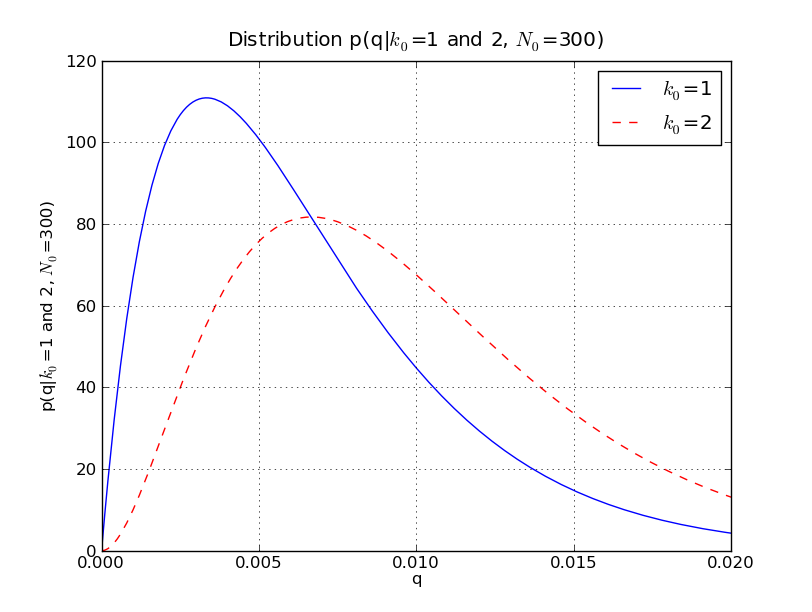
\includegraphics[scale=0.55]{Images/fap_distr.png}
\caption{Probability distribution function $p(q|k_0=1~\mathrm{and}~2,N_0=300)$ as a function of $q$. We notice that the maximum FAP, $q_0$, will increase with $k_0$, as expected; we also note that the width of the distribution increases with $k_0$, in other words, the FAP computation becomes less precise for events with higher maximum FAP.}
\label{fap_distr}
\end{figure}

\subsection{False Alarm Probability for $S$ Timeslides}

When prompted to assigning a certain false alarm probability to a candidate, one can artificially extend the background time, over which noise events can be gathered, by creating ``fake'' periods of data with approximately the same noise distribution as the real background data. This will keep the false alarm rate constant, but will allow us to make a more confident statement about a certain candidate by minimizing the error of the false alarm rate. This involves \emph{timesliding} the background data by a certain number of times, $S$, so that the new number of background trials will be $S \times N_0$. Physically, this is done by taking the detector data stretches and sequentially shifting one of them $S$ times by a certain amount of time $\Delta \tau$. By recombining the time--shifted data with the other non-slid segments, time--shifted triggers will form new coincident events. If the time--shifts $\Delta \tau$ are larger than the light travel time and the signal autocorrelation, then the time--shifted coincidences cannot be produced by gravitational waves, and are therefore expected to give a good estimate of the background -- from equation (\ref{far_c}) the coincidence rate is: 
%
\begin{equation}
\mathrm{FAR} = R_1R_2 \delta v
\label{thefar}
\end{equation}
%
and the variance will be, knowing that $S$ is the total number of timeslides, from \cite{Was:2009vh}:
%
\begin{equation}
\sigma = \sqrt{\sigma_{\mathrm{count}}^2 + \sigma_{\mathrm{recycled}}^2} = \sqrt{\frac{R_1R_2\delta v}{ST}+\frac{R_1R_2(R_1+R_2)\delta v^2}{T}}
\label{sigmatime}
\end{equation}
%
The first term of the sum represents ($\sigma_{\mathrm{count}}$) Poisson counting errors whereas the second term ($\sigma_{\mathrm{recycled}}$) represents the errors induced by repeating triggers forming different coincidences (``trigger recycling'', described in the following subsection). At low number of timeslides $S$, the counting errors will dominate the FAR error, whereas at higher $S$ values, the errors due to repeating triggers will dominate the magnitude of $\sigma$. This shows that the error will plateau if one increases the number of timeslides $S$ beyond a certain value, dependent on the single detector trigger rates $R_1$ and $R_2$ and the size of the coincidence window $\delta v$. In equation ~(\ref{sigmatime}), the number of timeslides at which the Poisson counting error term equals the repeating triggers error term:
%
\begin{equation}
\left ( \frac{R_1R_2\delta v}{ST} = \frac{R_1R_2(R_1+R_2)\delta v^2}{T} \right )_{S=S_{\mathrm{c}}}
\label{eq_saturation}
\end{equation}

\noindent will be improperly called the ceiling number of timeslides, $S_{\mathrm{c}}$. One may choose to do as many timeslides as one wants and there is no physical limit for $S$ simply imposed by the Poisson counting errors. It is just that by increasing the number of timeslides beyond $S_{\mathrm{c}}$ there is very limited gain in sensitivity. Hence, $S_{\mathrm{c}}$ follows from equation (\ref{eq_saturation}) and is given by:

\begin{equation}
S_{\mathrm{c}} = \frac{1}{(R_1+R_2) \delta v}
\label{timeslidesmax}
\end{equation}

By performing timeslides, we do not decrease the overall false alarm rate but rather decrease its error, compared to the case with no timeslides; the probability distribution function of the FAR will be peaked at the same maximum, but rather, the width will be smaller when doing timeslides.

GW detectors have different noise characteristics and local environmental influences, often resulting in very different trigger rates. It is useful to look at the accuracy of estimating the FAR when running an analysis with either very different detectors or similar ones, in terms of their individual trigger rates. We will be looking at equation (\ref{sigmatime}) that gives the FAR error $\sigma$ as a function of single detector trigger rates and number of timeslides and work with a constant FAR for both cases (it is only useful to assume a constant FAR to motivate a comparison of its error). Given two searches performed with two separate pairs of detectors, at a constant FAR and fixed number of timeslides $S$, we can differentiate two analysis cases: one that uses almost identical detectors, hence equal trigger rates $R_1 \approx R_2 = R$ and another that uses two very different detectors, with two very different trigger rates, e.g., $R_2 = f \times R_1$, where $f<1$ is an arbitrary proportionality factor. Since we are working at a fixed FAR, in equation (\ref{sigmatime}), the first term of the sum will be constant for both analyses, for the same number of $S$ timeslides. We need to compare the second term, namely $R_1+R_2 = (1+f) R_1$ with $2R$. We have the relation between $R_1$ and $R$, given a constant FAR: 
%
\begin{equation}
FAR = R_1R_2\delta v = fR_1^2 \delta v = R^2 \delta v
\end{equation}
%
hence $R=f^{1/2}R_1$. Replacing in equation (\ref{sigmatime}), we obtain the ratio of the two FAR errors in the two cases, for a fixed number of timeslides $S$:
%
\begin{equation}
\frac{\sigma_{R_1 \gg R_2}}{\sigma_{R_1=R_2=R}} = \sqrt{\frac{1+(1+f)SR_1 \delta v}{1+2\sqrt{f}SR_1 \delta v}}
\label{fractionalerror}
\end{equation}
%
For an arbitrary number of timeslides, e.g., $SR_1 \delta v=1$ (a low number of timeslides $S$=100, a relatively high trigger rate $R_1$=10 Hz and a typical estimated value $\delta v = 10^{-3}$ s), constant for both cases, we have the ratio as function of the proportionality factor $f$:
%
\begin{equation}
\frac{\sigma_{R_1 \gg R_2}}{\sigma_{R_1=R_2=R}} = \sqrt{\frac{1+(1+f)}{1+2\sqrt{f}}}
\end{equation}
%
For $f \rightarrow 0$ we expect an increase of roughly 50\% of the error on the false alarm rate when performing an analysis with two detectors with very different trigger rates as compared to one with similar trigger rates, for a given number of timeslides and a fixed FAR. In conclusion, the ability to measure the FAR is reduced when using two detectors with very different trigger rates; in such a case, we would be more susceptible to removing true signals, if present in the data. This effect is much enhanced when performing a considerable number of timeslides, e.g., of order $10^6$ (not applicable in the case of a GRB analysis where we have data stretches of only 2000s, but where we have longer data segments). In this case the dominant term will be $SR_1 \delta v$ of order $10^4$ and the ratio of FAR errors will be of order $(1+f)/(2 \sqrt{f}) \gg 1$ for small values of $f$. This effect is sensitive to values of single detector trigger rates: in the case of an analysis with very low trigger rates, e.g., $R_1 \approx 10^{-3}$, this effect may be neglected since $SR_1 \delta v \ll 1$ and the errors will be approximately equal: in equation (\ref{fractionalerror}) for small $f$ values the numerator and denominator sums will $\rightarrow$ 1.

To conclude, when dealing with relatively high single detector trigger rates, the timeslid background is better estimated (FAR error is smaller) when using data from detectors with similar trigger rates values, as opposed to very different trigger rates.

\subsection{Different scenarios for FAP and error}
\paragraph{Fixed time--mass coincidence window}
For a typical coincident GW--GRB analysis the single detector trigger rates close to threshold SNR are relatively high at values of order $R_1 \approx R_2 \approx 100$ triggers/second; using a constant coincidence window of order $\delta v \approx 10^{-3}$ s and a total number of trials $N_0 = 300$ with an ``on--source'' length of $T=6$~s, we can estimate what false alarm probabilities we would expect from three different classes of triggers, ranked solely by their characteristic SNR values (identical background triggers with different loudness): with low SNR, close to threshold, medium SNR and high SNR. Triggers with low SNR will have a high occurrence rate, whereas triggers with high SNR will have a low occurrence rate. Table \ref{xes} summarizes the false alarm rates and errors for these cases, for two types of analysis: without timeslides (``zero--lag'' only) and with S=100 timeslides. Trigger rates $R_1$ and $R_2$ are used in equations (\ref{thefar}) and (\ref{sigmatime}) to calculate the FAR and its error, $\sigma$; also in equation (\ref{timeslidesmax}) to estimate the ceiling number of timeslides, $S_{\mathrm{c}}$.

\begin{table}[ht!]
 \begin{tabular}{|l|l|l|l|l|l|}
 \hline
 \hline
 $R_1$ (Hz) & $R_2$ (Hz) & FAR (Hz) & $\sigma_{\mathrm{FAR}}$ (Hz) S=0 & $\sigma_{\mathrm{FAR}}$ (Hz) S=100 & $S_{\mathrm{c}}$ \\
 \hline
 100 & 100 & 10 & 1.3 & 0.60 & $<$1 \\
 10 & 10 & 0.1 & 0.13 & 0.02 & 50 \\
 1 & 100 & 0.1 & 0.13 & 0.04 & 10\\
 1 & 1 & 0.001 & 0.013 & 0.001 & 500 \\
 1 & $10^{-2}$ & $10^{-5}$ & $1.3 \times 10^{-3}$ & $1.3 \times 10^{-4}$ & $5 \times 10^3$ \\
 $10^{-2}$ & $10^{-2}$ & $10^{-7}$ & $1.3 \times 10^{-4}$ & $1.3 \times 10^{-5}$ & $5 \times 10^4$ \\
 $10^{-3}$ & $10^{-3}$ & $10^{-9}$ & $1.3 \times 10^{-5}$ & $1.3 \times 10^{-6}$ & $5 \times 10^5$ \\
 \hline
 \hline
 $R_1$ (Hz) & $R_2$ (Hz) & FAR (Hz) & $\sigma_{\mathrm{FAR}}$ (Hz) S=0 & $\sigma_{\mathrm{FAR}}$ (Hz) S=$10^3$ & $S_{\mathrm{c}}$ \\
 \hline
 $10^{-3}$ & $10^{-3}$ & $10^{-9}$ & $1.3 \times 10^{-5}$ & $1.3 \times 10^{-7}$ & $5 \times 10^5$ \\
 \hline
 \hline
 \end{tabular} 
 \caption{False alarm rates and their errors for different combinations of trigger rates for a simple two--detector analysis in the cases of ``zero--lag'' (no timeslides, S=0) and S=100 timeslides. Trigger rates $R_1$ and $R_2$ are used in equations (\ref{thefar}) and (\ref{sigmatime}) to calculate the FAR and its error, $\sigma$; also in equation (\ref{timeslidesmax}) to estimate the ceiling number of timeslides, $S_{\mathrm{c}}$. This illustrates the gain in confidence from a low--and--equal--trigger rates case. The very low trigger rates cases imply that the false alarm rate can be quoted only as a confidence interval [$-\sigma,\sigma$] that approaches [$-10^{-6}, 10^{-6}$] for trigger rates in the mHz region. We repeat the last row in the second section of the table; this is motivated by a choice of very low single detector trigger rates allowing the performance of a considerable amount of timesliding ($S=10^3$, permitted by equation (\ref{timeslidesmax})), in the case of an analyzed stretch of 2000 s, that, in turn, combined with very low and roughly equal single detector trigger rates (mHz), contribute to significantly lowering the $\sigma$ value of the FAR to reach $\approx 10^{-9}$ Hz and its error $\approx 10^{-7}$ Hz.}
 \label{xes}
\end{table}

By examining Table \ref{xes} we can draw a series of conclusions with regards to the usability of timeslides to estimate false alarm probabilities:
\begin{itemize}
\item
The coincidence rate for triggers with low SNR, close to threshold, is high and the timeslides method is indeed improving the FAR error but the large number of such coincidences would render any ``on--source'' trigger resembling them, completely insignificant. The FAR may have values of order 10 Hz and the ceiling number of timeslides is below 1, implying it is useless to do timeslides when we only have such triggers (see row 1 of the Table \ref{xes}).
\item
A factor contributing towards the increase of FAR error is two very different trigger rates in the two detectors, when dealing with relatively high trigger rates values (see rows 2 and 3 of the Table \ref{xes}). This effect is completely described by equation (\ref{fractionalerror}), that quantifies the fractional increase of the error for any given $S$ timeslides. The effect of two very different values for single detector trigger rates is of roughly 50\% increase in $\sigma$ for an analysis with a given $S$ timeslides and may increase significantly for analyses with much larger number of timeslides and high single detector trigger rates; note that for low $S$ and $R_1$, the effect is not so strong and the errors are approximately equal; also it suffices to consider the case of higher $S$ and not do a full analysis depending on the values of $S$ since a more exact background estimation for a GRB search will need higher values for $S$, i.e., $SR_1\delta v \gg 1$. The effect of two very different values for single detector trigger rates is less noticeable for low values of the single detector trigger rates, e.g., of order mHz, and relatively low number of timeslides. Ideally, an analysis should make use of two similar detectors in terms of trigger rates. This, combined with a low value of trigger rates, will allow for a smaller error value and for a larger number of usable timeslides.
\item
The coincidence rate for triggers with high SNR is low and in this case the timeslides method does improve the FAR error by an order of magnitude. Yet due to counting errors and repeating triggers, the error, even by performing 100 timeslides, is still of the same order of magnitude as the FAR (see row 4 of Table \ref{xes}).
\item
We can still achieve false alarm rates in the desired region of $10^{-6}-10^{-8}$ by performing timeslides if we have a very low individual detector trigger rate and the rates from any two detectors are comparable (at least of the same order of magnitude) (see rows 5,6 and 7 of the Table \ref{xes}; also the second section of Table \ref{xes}).
\end{itemize}

\subsection{Time--mass coincidence window function of threshold SNR}
As we see from Table \ref{xes} one would ideally want a very low trigger rate in the detector data. This can be achieved by very effective glitch--reduction procedures (effective detector characterization), very strong signal--based vetoes and by raising the SNR threshold. Glitch--rejection and signal--based vetoes tend to reduce the number of loud noise events and not to reduce the background of near--threshold ones. We will briefly discuss the third option: raising the SNR threshold $\rho_0$ that will significantly reduce the number of low--SNR noise events. Using equation (\ref{xellipse0}), we can write the FAR and its error as a function of threshold SNR $\rho_0$:
%
\begin{equation}
FAR(\rho_0) = \frac{0.11R_1R_2}{\rho_0^3}
\end{equation}
%
and
%
\begin{equation}
\sigma = \sqrt{\frac{0.11R_1R_2}{ST\rho_0^3}+\frac{10^{-2}R_1R_2(R_1+R_2)}{T\rho_0^6}}
\end{equation}
%
Also, suppose we assume, in a very approximate case, that the single detector trigger rates are equal and decrease as exponential functions of threshold SNR:
%
\begin{equation}
R_1 \approx R_2 \approx C\mathrm{e}^{-\alpha \rho_0}
\end{equation}
%
where $C$ and $\alpha$ are two analysis--dependent constants that we can evaluate and approximate fixed for similar analyses. This naive approximation is not very far from reality in the ideal case of a stretch of data without any major non--Gaussian noise activity. The constant $C$ can be evaluated using the trigger numbers from Chapter \ref{Chapter Four} for the case of GRB090809B: at a threshold SNR $\rho_0=4.5$ the single detector trigger rates were in the region of 50 Hz, giving us an estimate $C=3 \times 10^{10}$ Hz. The constant $\alpha$ can be evaluated knowing that there is order 100 drop in FAR for a unit increase in SNR, so roughly $100 \approx \mathrm{e}^{\alpha}$, giving $\alpha \approx 4.5$. This way we can re--write both the FAR and its error taking this into account:
%
\begin{equation}
FAR(\rho_0) = 9 \times 10^{18} \times \frac{\mathrm{e}^{-2 \alpha \rho_0}}{\rho_0^3}
\end{equation}
%
and
%
\begin{equation}
\sigma = 3 \times 10^9 \times \sqrt{\frac{\mathrm{e}^{-2 \alpha \rho_0}}{ST\rho_0^3}+6 \times 10^{10}\frac{\mathrm{e}^{-3 \alpha \rho_0}}{T\rho_0^6}}
\end{equation}
%
with a ceiling number of timeslides as a function of threshold SNR:
%
\begin{equation}
S_c \approx 1.7 \times 10^{-11}\rho_0^3\mathrm{e}^{\alpha \rho_0}
\end{equation}
%
The false alarm rate and its error are shown in Figure \ref{FAR_threshold}: false alarm rate variation with threshold SNR $\rho_0$ (continuous line) and its error (dashed lines) for $T=6$ s and a sequence of $S=10^n$ timeslides where $n=\bar{0,11}$; vertical lines corresponding to a sequence of $\rho_0$=5, 6, 7, 8 and 9, in a log--log plot. The dashed contours representing the $\sigma$ of the FAR, for constant number of timeslides, reveal two very important findings: the error saturates and does not decrease anymore even if we would perform an infinite number of timeslides (this was also shown in equation (\ref{eq_saturation}), explaining the existence of a ceiling number of timeslides, above which there is no decrease in error); and justifies the performance of timeslides in order to obtain a reduced error on the false alarm rate: the error decreases with increasing $S$.

\begin{figure}[ht!]
%\begin{minipage}[b]{0.5\linewidth}
\centering
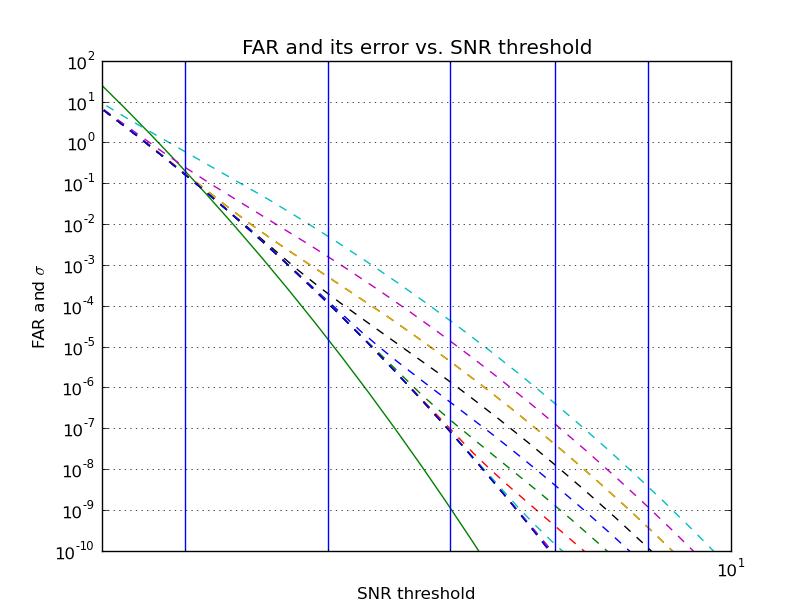
\includegraphics[scale=0.55]{Images/far_threshold1.png}
\caption{False alarm rate variation with threshold SNR $\rho_0$ (continuous line) and its error (dashed lines) for $T=6$ s and a sequence of $S=10^n$ timeslides where $n=\bar{0,11}$, the furthest error line from the FAR line is for $n=0$ and the closest for $n=11$; vertical lines corresponding to $\rho_0$=5,6,7,8 and 9, log--log plot. The dashed contours representing the $\sigma$ of the FAR, for constant number of timeslides, reveal two very important findings: the error saturates and does not decrease anymore even if we would perform an infinite number of timeslides (this was also mentioned in equation (\ref{eq_saturation}), explaining the existence of a ceiling number of timeslides, above which there is no decrease in error); and justifies the performance of timeslides in order obtain a reduced error on the false alarm rate: the error decreases with increasing $S$.}
\label{FAR_threshold}
%\end{minipage}
%\hspace{0.5cm}
%\begin{minipage}[b]{0.5\linewidth}
%\centering
%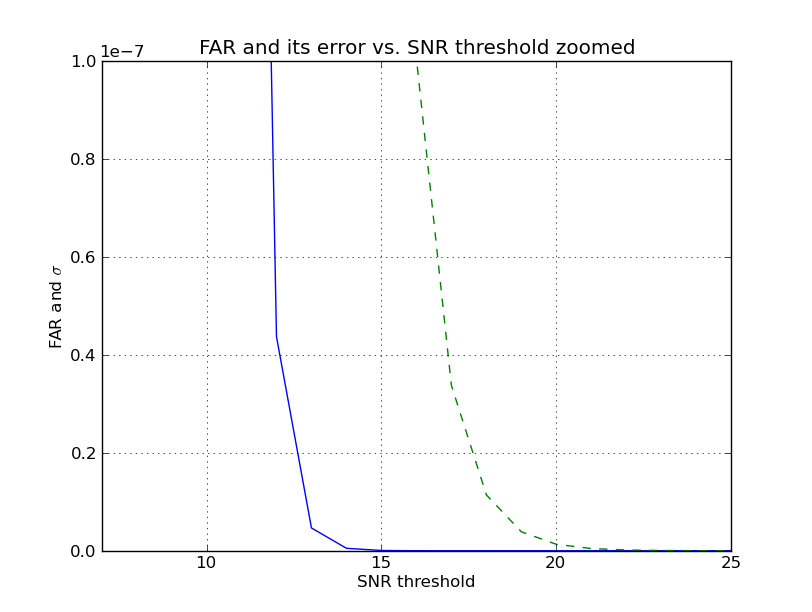
\includegraphics[scale=0.40]{Images/FAR_threshold_zoom.png}
%\caption{False alarm rate variation with threshold SNR (continuous line) and its error (dashed line) in the region of interest for the FAR of a GW--GRB search. The error is roughly two orders of magnitude larger than the FAR.}
%\label{FAR_threshold_zoom}
%\end{minipage}
\end{figure}

Looking at a practical case: suppose we impose a threshold SNR $\rho_0=7$, or consequently, we have two coincident triggers, each with SNR's 7 -- this would mean an effective SNR of $\approx$10, which would probably mean the loudest event in the case of a GW--GRB search. The coincident event will have a FAR$\approx 10^{-9}$ and the error on the FAR will be $\sigma \approx 10^{-4}$ for S=1 timeslides (``zero--lag''+1 slide only) and $\sigma \approx 10^{-7}$ for S=$10^3$ timeslides (possible for a 2000 s data stretch), already becoming of interest given the very low probability of finding a short GRB located within the GW detectors' range, equation (\ref{grb_p}).

\subsection{Repeating triggers and trigger occurrence rates} 

A coincidence, as used in the above formulation, is constructed from two individual detector triggers, found within a certain coincidence window. Up to now, we have not made any statements about the uniqueness of these single detector triggers, when performing timeslides. When performing an analysis of the ``zero--lag'' these triggers should ideally be unique for every coincidence for every detector. When timeshifting the data, the same single detector triggers may participate in numerous coincidences, since the timeslides method of ``extending'' the background does not produce new triggers but rather \emph{reuses} the same triggers within the analysis time $S \times N_0 \times T$ to create new coincidences at every slide step. We will assume the same simple case as before: coincident data from two different GW detectors, with trigger rates $R_1$ and $R_2$, respectively. Assuming that, within a coincidence window $\delta v$, a trigger from detector 1 has equal probability to form a coincidence with any trigger from detector 2, we define the average expected occurrence $z_1$ of a given trigger from detector 1 in timeslid coincidences with triggers from detector 2 as:
%
\begin{equation}
\label{occrate1}
z_1(R_2) = R_2 S \delta v
\end{equation}
%
The probability that any trigger from detector 1 will form $k$ coincidences when doing an analysis comprising $S$ timeslides may be approximated with a Poisson process probability with a constant occurrence $z_1$:
%
\begin{equation}
\label{poissontriggers}
p_1(k|z_1) \rightarrow p_1(k|R_2) = \frac{z_1^k}{k!} \mathrm{e}^{-z_1} = \frac{{(R_2 S \delta v)}^k}{k!} \mathrm{e}^{-R_2 S \delta v}
\end{equation} 
%
If in real data, the trigger occurrence is Poisson distributed, that means there is no preference that certain triggers should occur more often than others, i.e. all the triggers belong to the same statistical sample and there is no correlation between trigger times. This is not always true: triggers associated with detector glitches tend to show up in many more coincidences than triggers associated with Gaussian noise; if the background was purely Gaussian, the occurrence distribution would be Poissonian. We would like to investigate this for a test analysis. 
%
\begin{figure}[ht!]
%\begin{minipage}[b]{0.5\linewidth}
\centering
%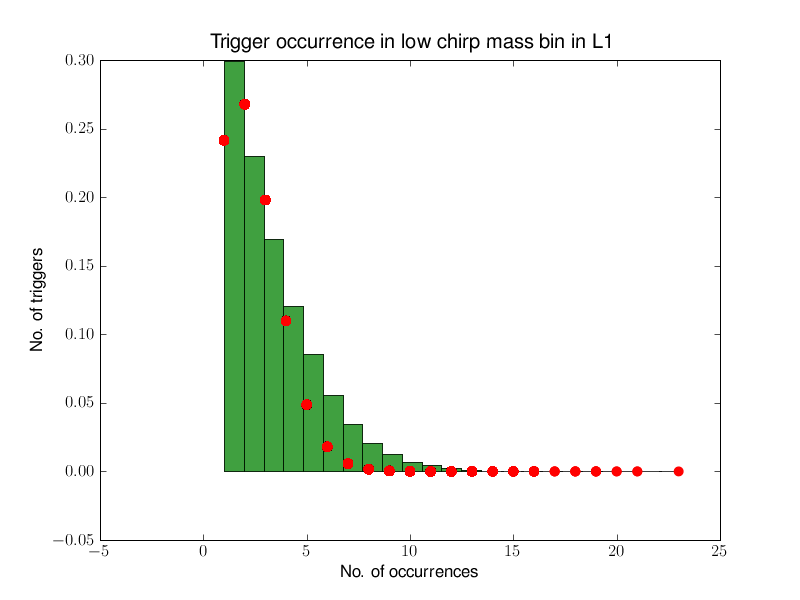
\includegraphics[scale=0.45]{Images/l1_low_distribution.png}
%\caption{Histogram of number of trigger occurrences in coincidences for GRB090809B: detector 1, low chirp mass bin (L1low)}
%\label{figure4}
%\end{minipage}
%\begin{minipage}[b]{0.5\linewidth}
\centering
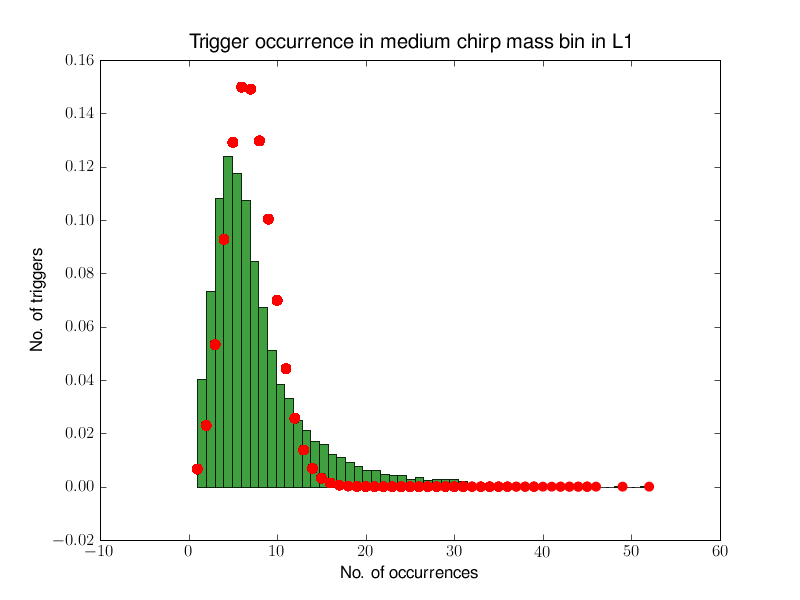
\includegraphics[scale=0.55]{Images/l1_medium_distribution.png}
%\caption{Histogram of number of trigger occurrences in coincidences for GRB090809B: detector 1, medium chirp mass bin (L1medium)}
%\label{figure5}
%\end{minipage}
%\begin{minipage}[b]{0.5\linewidth}
%\centering
%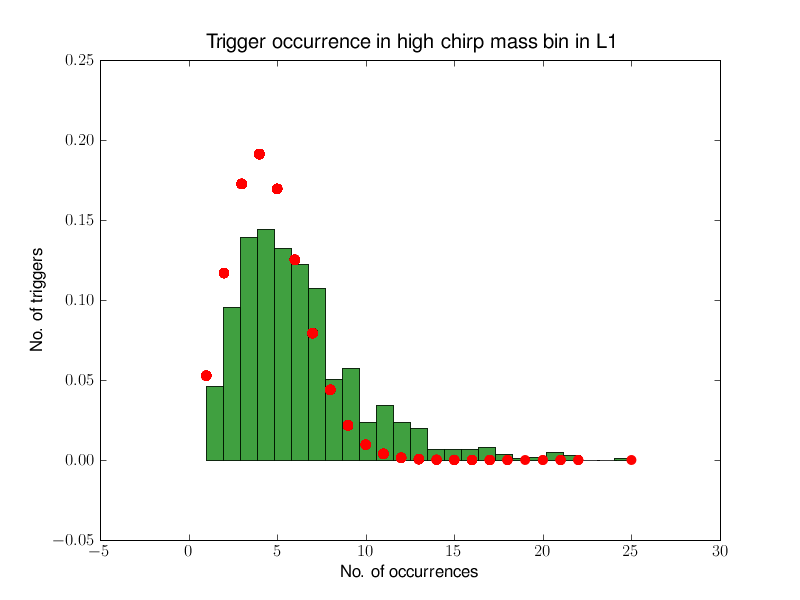
\includegraphics[scale=0.45]{Images/l1_high_distribution.png}
%\caption{Histogram of number of trigger occurrences in coincidences for GRB090809B: detector 1, high chirp mass bin (L1high)}
%\label{figure6}
%\end{minipage}
%\begin{minipage}[b]{0.5\linewidth}
%\centering
%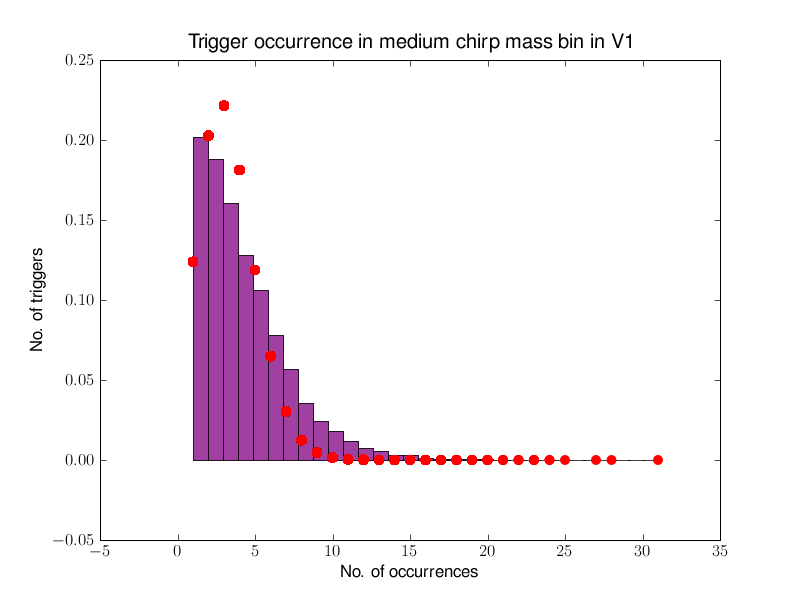
\includegraphics[scale=0.45]{Images/v1_medium_distribution.png}
%\caption{Histogram of number of trigger occurrences in coincidences for GRB090809B: detector 1, medium chirp mass bin (L1medium)}
%\label{figure5}
%\end{minipage}
\caption{Histogram of number of trigger occurrences in coincidences for a test GW--GRB coincident analysis with $S=160$ timeslides (for one of the detectors; normalization factor of 300 on the $y$--axis). Fitted (the dots) is the theoretical (expected) Poisson distribution of the number of occurrences, given by equation (\ref{poissontriggers}). The theoretical Poisson fit overestimates the number of triggers with low occurrence and underestimates the number of triggers with higher occurrence. This can be explained by correlations in trigger times due to non--Gaussian ``glitches''. We do not, however, notice a significant deviation from the predicted distribution; the expected occurrence for a fixed single detector trigger rate of 50 Hz, coincidence window width of $10^{-3}$ and 160 timeslides is $z=8$; the histogram peaks at roughly 5 occurrences.}
\label{poissonD}
\end{figure}

Figure \ref{poissonD} is a histogram of number of trigger occurrences in coincidences for a test GW--GRB coincident analysis with $S=160$ timeslides (for one of the detectors). Fitted (the dots) is the theoretical (expected) Poisson distribution of the number of occurrences, given by equation (\ref{poissontriggers}). The theoretical Poisson fit overestimates the number of triggers with low occurrence and underestimates the number of triggers with higher occurrence. This can be explained by correlations in trigger times due to non--Gaussian ``glitches''. Another explanation for these deviations is the choice of statistic for the model: a binomial distribution might be more suited to fit the histogram, since the Poisson distribution is an approximation of the binomial distribution. We do not, however, notice a significant deviation from the predicted distribution (whether it be Poisson or binomial); the expected occurrence for a fixed single detector trigger rate of 50 Hz, coincidence window width of $10^{-3}$ and 160 timeslides is $z=8$; the histogram peaks at roughly 5 occurrences. Since we would not have any reason to consider triggers be correlated, such a Poisson test--fit would be useful to identify the triggers that occur more than expected, thus finding correlations between triggers.

\subsection{Conclusions}
The chance that the distance to a short GRB is within the initial GW detector range is very low; we have used a very naive estimation of this chance probability and shown that it is of order $10^{-6} - 10^{-7}$. Given this, in order for a GW event, associated with a short GRB with no redshift measurement, to be considered a detection, its false alarm probability should be of order $10^{-6} - 10^{-7}$. We are unable to obtain such low FAP from the analysis of a single background GW data stretch for a GW--GRB analysis. Therefore we timeshift the data to create more coincident background. We have examined the simplest case of two coincident data stretches from two different GW detectors, with different trigger rates. We have estimated the size of a coincidence window and using this we have derived expressions for the background false alarm rate and its error, when timeshifting the data. Given a loud ``on--source'' event, the timeslides method may reduce the FAR error to a confidence interval that allows us to consider it a detection. The timeslides method is most efficient when working with detectors with similar trigger rate values. Imposing a higher SNR threshold will also add to this improvement by reducing the individual detector trigger rates and allowing for a larger number of timeslides to be performed. We have also shown that repeating single detector triggers in timeslid coincidences follow a distribution that resembles a Poisson distribution; such a distribution test may be used to identify non--Gaussian triggers that tend to show up in multiple coincidences across the timeslid background.

\section{Implementing timeslides in the analysis pipeline}

In the previous section we have shown theoretically that by performing timeslides we may be able to restrict the false alarm rate and probability to a confidence interval small enough to be comparable to an astrophysical probability that quantifies the chance a GRB was within the GW detectors' range. In the next section we will present how we implemented and tested the timeslides method in the case of an actual analysis.

\subsection{Test GRB}

The testing to implement timeslides in the coincident GRB analysis was done on an S6/VSR2 and 3 long GRB observed by Fermi--GBM, GRB090809B (trigger time GPS 933895709, date and time August 09 2009, 23:28:14 UTC, sky location RA=95.3, deg=0.1 degrees) \cite{gcn9760}. GRB090809B had available coincident data from Livingston L1 and Virgo V1. An inspection of the number of triggers participating in second--stage coincidences as function of SNR (Figure \ref{V1triggers}) reveals an exponential decrease with a long high--SNR tail and a high number of triggers near threshold ($\rho_0=4.5$); the high--SNR tail represents the population of ``glitches'' that reveal a non--Gaussian background.

\begin{figure}[ht]
\begin{minipage}[b]{0.5\linewidth}
\centering
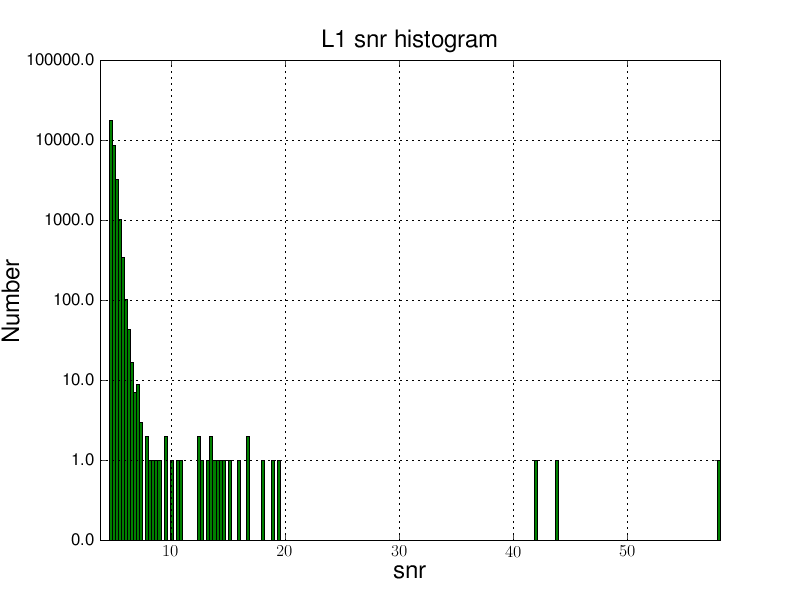
\includegraphics[scale=0.40]{Images/l1_triggers.png}
%\caption{Histogram of L1 triggers that participate in second--stage coincidences as function of SNR for GRB090809B. The majority of the triggers are at low SNR, near threshold; a tail of high--SNR ``glitches'' is present, revealing a non--Gaussian distribution of trigger events.}
%\label{L1triggers}
\end{minipage}
\hspace{0.5cm}
\begin{minipage}[b]{0.5\linewidth}
\centering
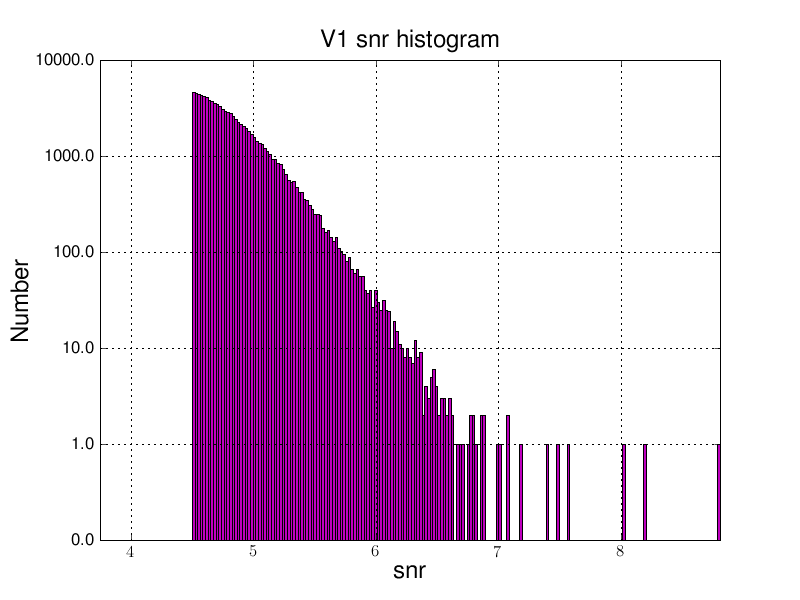
\includegraphics[scale=0.40]{Images/v1_triggers.png}
\end{minipage}
\caption{Left figure: histogram of L1 triggers that participate in second--stage coincidences as function of SNR for GRB090809B. The majority of the triggers are at low SNR, near threshold; a tail of high--SNR ``glitches'' is present, revealing a non--Gaussian distribution of trigger events. Right figure: histogram of V1 triggers that participate in second--stage coincidences as function of SNR for GRB090809B. The majority of the triggers are at low SNR but in this case the spread is more even across the SNR values with a much shorter tail of ``glitches''.}
\label{V1triggers}
%\end{minipage}
\end{figure}

\subsection{Implementation of timeslides}
The implementation of the timeslides analysis is fairly straightforward and uses the same basic principle as used in the previous all--sky searches \cite{Abbott:2009dk, Abadie:2010yba}. Given two arbitrary GW detectors $A$ and $B$, we can imagine the data from these detectors as rings and by fixing, say, detector $A$ data ring and rotating detector $B$ data ring by a certain \emph{slide amount}, a finite number of times, so that we will obtain new coincidence data. We keep rotating the detector $B$ ring until reaching the initial 0 position. In practice, this is done by translating in time--domain the data from one detector by a certain time amount $\Delta t$ with respect to the other (fixed in time) data from the other detector, making sure to re--attach the outstanding segment $\Delta t$ at the other end of the time--shifted detector data. By performing a finite $S$ number of such time--shifts of the data segments and repeating the coincidence tests described in Chapter \ref{Chapter Four} for every of the $S$ time--shifts, new coincidences are found and the background is sampled more finely as explained above.

Since for every timeslide $S$ we repeat the coincident stage of the pipeline, we will inherently obtain $S$ new lists of coincidences that should be clustered on trial and chirp mass in order to find the loudest coincident event in each of these trials, as explained in Chapter \ref{Chapter Four}, and masked for vetoing the trials that should be removed due to data quality reasons. The trial clustering and vetoes application is illustrated in Figure ~\ref{slidesGRB} and detailed below.

\begin{figure}[ht!]
\centering
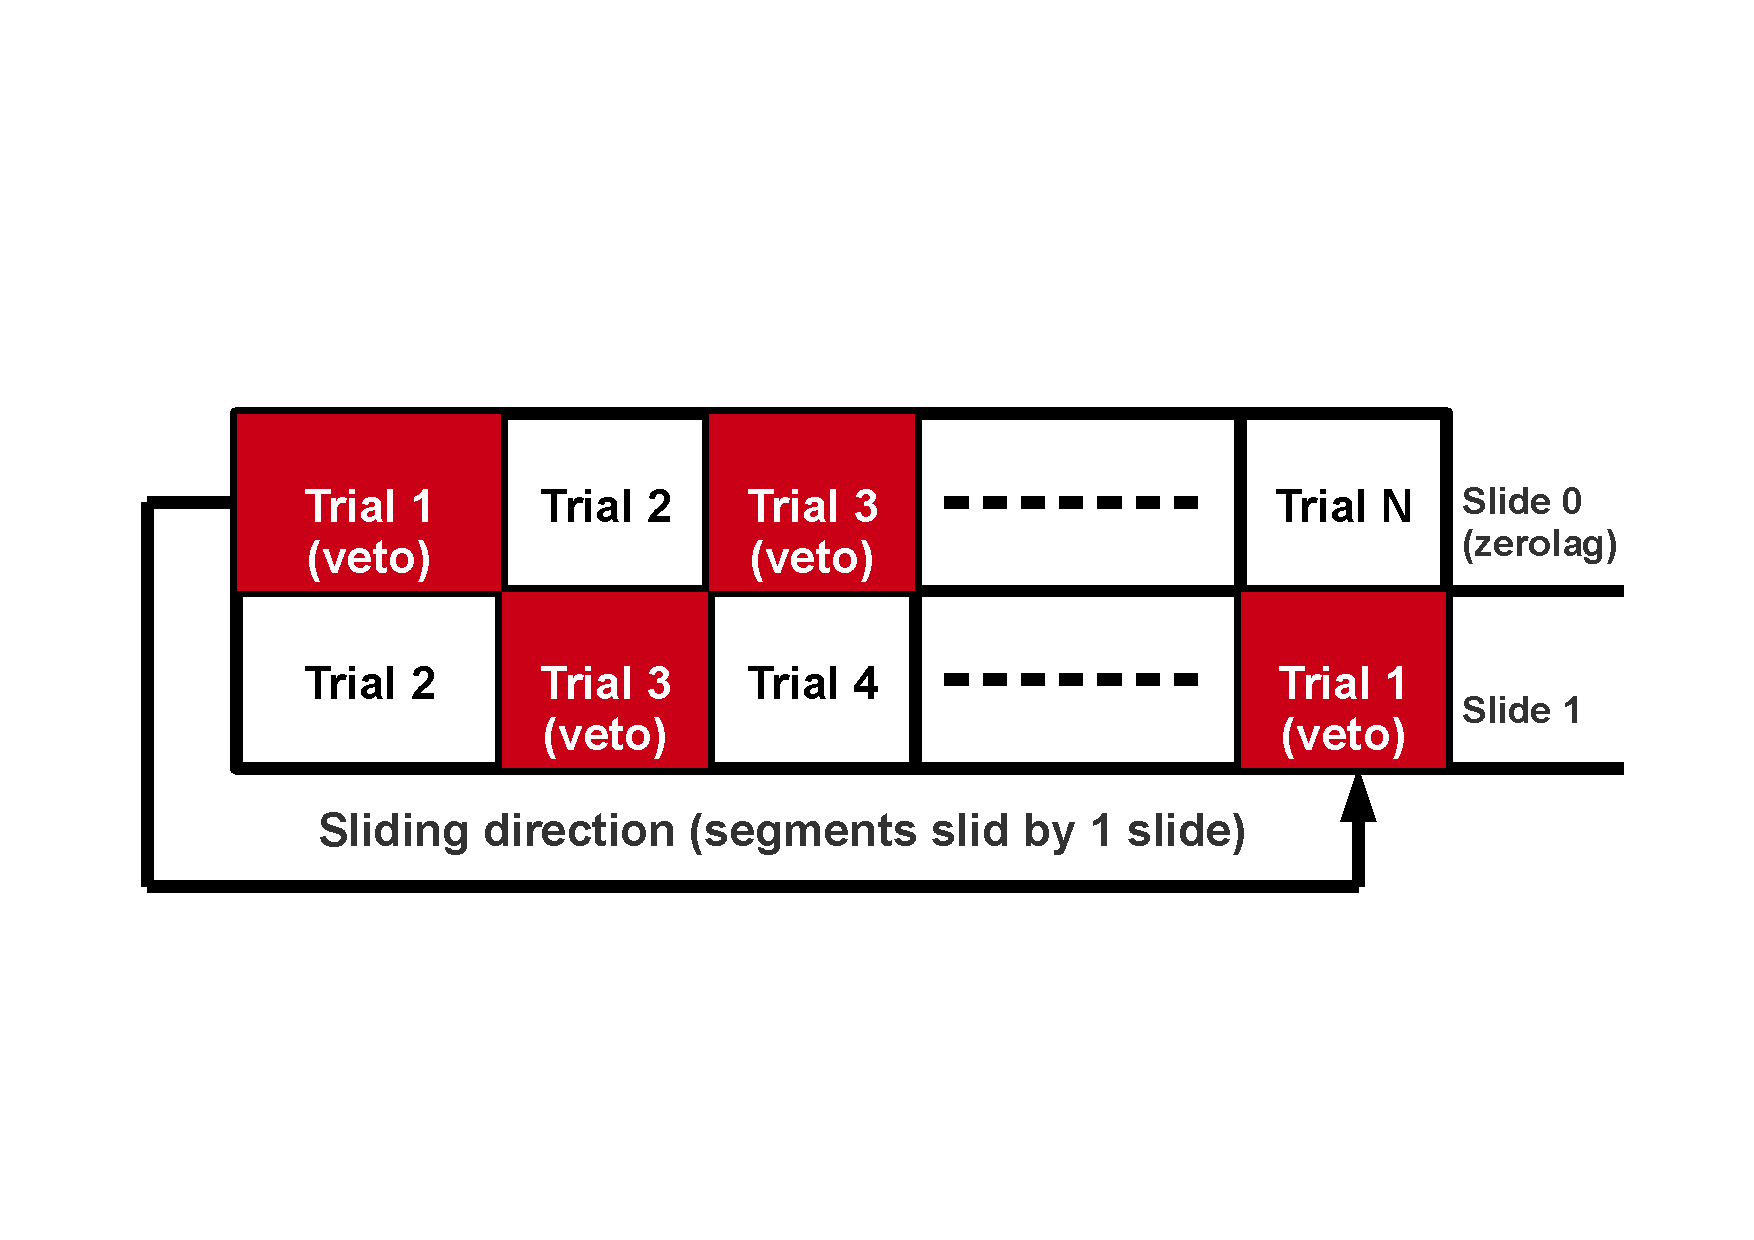
\includegraphics[scale=0.45]{Images/SlidingGRB.pdf}
\caption{Two--dimensional trial--slide veto mask designed to cluster coincidences in 6--s trials and apply vetoes in the case of a GRB analysis with timeslides: veto times (times of bad detector data) are overlapped with the ``zero--lag'' (Slide 0) that is partitioned in 6--s trials; the trials that fall during the veto times are marked as unwanted (full color here in the figure, example Trial 1) and none of the coincidences found in these trials will be considered for analysis. The first slide is built by timeshifting by a certain amount (usually multiples of 6--s, exactly 6--s in this figure, or the length of a trial) the whole ``zero--lag'' and re--attaching the remainder to the other end of the data stretch (Trial 1 here); the second slide is built in the same manner with reattaching the remainder (here it would be Trial 2) and so on. After $S$ timeshifts we will have a 2--dimensional (in trial along one dimension and slide number along the other) mask populated with valid and vetoed trials. We apply this mask to the actual time--shifted GW data and retain only the coincidences found in the un--vetoed trials.}
\label{slidesGRB}
\end{figure}

The coincident lists obtained from an analysis (matched--filtering, coincidence tests) with timeslides are stacked hierarchically starting from slide 0 (``zero--lag'') to slide $S$. At this stage we will partition each of these lists into 6--second trials, just as we would do in the case of a ``zero--lag'' analysis. We will want to discard the times of excessively noisy data by applying the data quality vetoes (as described in Chapter \ref{Chapter Four}, category two vetoes). The times to be vetoed are found in text lists parameterized by the start and end times of each of the bad data sectors. We overlap this list in time domain with the 0th slide (the ``zero--lag'') and mark each of the 6--s trials that fall during the vetoed times as unwanted; if a certain vetoed interval accounts for a non--integer number of 6--s trials, we discard all the trials that contain any veto times. This is done independently for every detector data. This will provide us with a 1--dimensional mask partitioned in 6--second trials that are either to contain coincident triggers to be taken account of in the analysis or to be discarded due to bad detector data. So far we have done this only for the 0th slide; sliding this mask with a certain slide amount for each timeslide will provide us with a two--dimensional trial--slide mask, populated with either empty timeshifted trials or with timeshifted veto trials. Coincidences falling in the vetoed trials are discarded, whereas those falling in a un--vetoed trial are kept.

\subsection{Test GRB results}
First, the background without timeslides (``zero--lag'') has been estimated and is shown in Figure \ref{datimeslides} (left). This is a cumulative histogram of background coincidences louder than a given SNR. Then the background obtained by doing $S=160$ timeslides has been estimated and is shown in Figure \ref{datimeslides} (right). The decrease in the FAP for background events is of order $\approx$160 (since we performed timeslides only for the off--source and we slid on two rings of 80 timeslides each), roughly the number of timeslides we performed.

\begin{figure}[ht!]
\begin{minipage}[b]{0.5\linewidth}
\centering
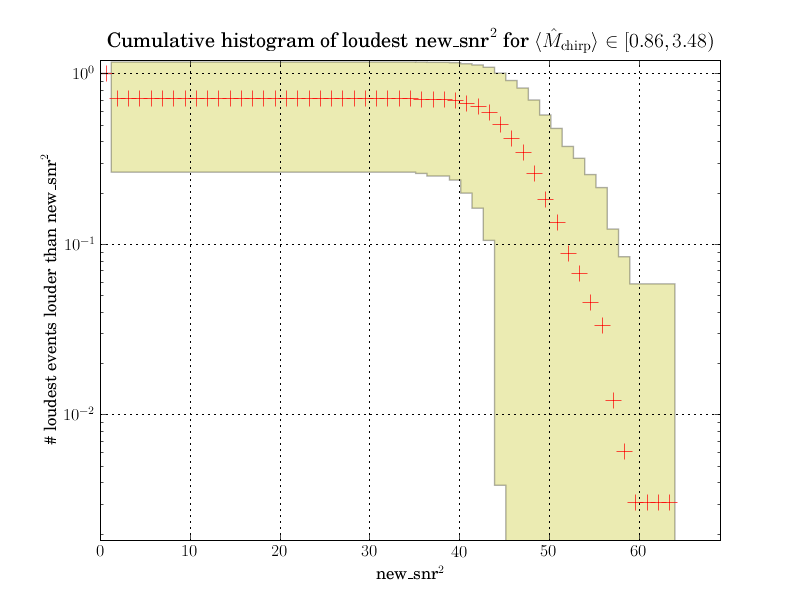
\includegraphics[scale=0.40]{Images/GRB090809B_lowmass_NOslides.png}
%\caption{Cumulative histogram of the loudest background events in the ``zero--lag'' case in the low chirp mass bin. The ``loudest'' events (highest effective SNR) populate the tail of the distribution at FAP of order 1/300.}
%\label{niettimeslides}
\end{minipage}
\hspace{0.5cm}
\begin{minipage}[b]{0.5\linewidth}
\centering
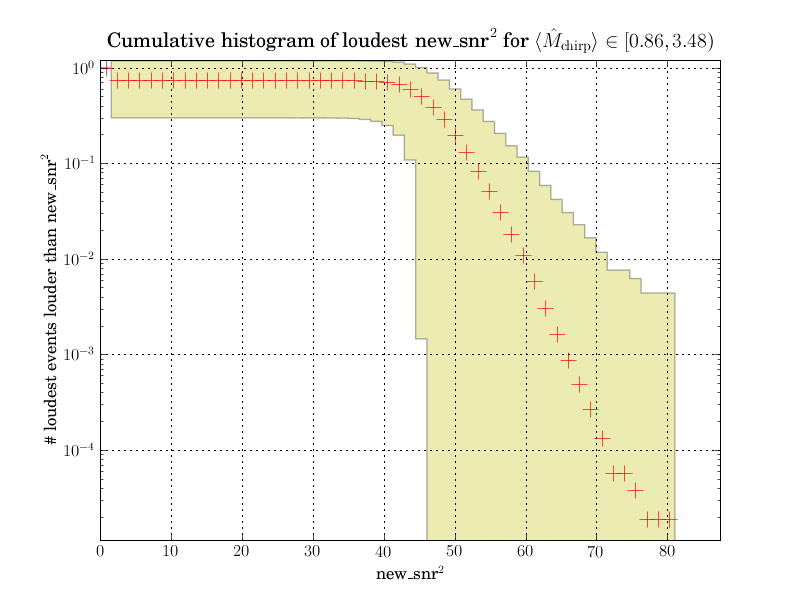
\includegraphics[scale=0.40]{Images/GRB090809B_lowmass_80slides.png}
\end{minipage}
\caption{Cumulative histogram of the loudest background events: left figure in the ``zero--lag'' case in the low chirp mass bin -- the ``loudest'' events (highest effective SNR) populate the tail of the distribution at FAP of order 1/300; right figure in the timeslides (160 timeslides) case in the low chirp mass bin -- the ``loudest'' events (highest effective SNR) populate the tail of the distribution at FAP of order 1/$300 \times 160$$\approx 2 \times 10^{-5}$.}
\label{datimeslides}
%\end{minipage}
\end{figure}

Estimating the background using timeslides does not change the overall average background distribution since most of the coincidences are consisted of low--SNR triggers that will produce more and more low--SNR coincidences once timeslides are performed. Timeslides add to the loud--SNR tail though; the larger the number of timeslides is the larger the chances to have loud events in the tail, louder than the ``zero--lag'' loudest triggers, as shown in Figures \ref{090809B_onsource_slides} (left) and \ref{090809B_onsource_slides} (right). 

\begin{figure}[ht!]
\begin{minipage}[b]{0.5\linewidth}
%\centering
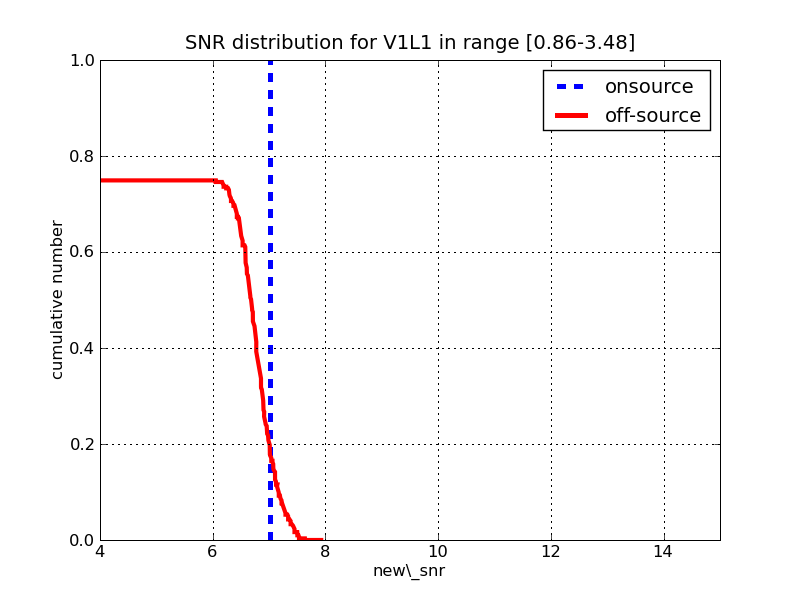
\includegraphics[scale=0.40]{Images/090809B_onsource_noslides.png}
%\caption{Background distribution (continuous line) and loudest on--source event (dashed line) when no timeslides are performed (``zero--lag'').}
%\label{090809B_onsource_noslides}
\end{minipage}
%\hspace{0.5cm}
\begin{minipage}[b]{0.5\linewidth}
%\centering
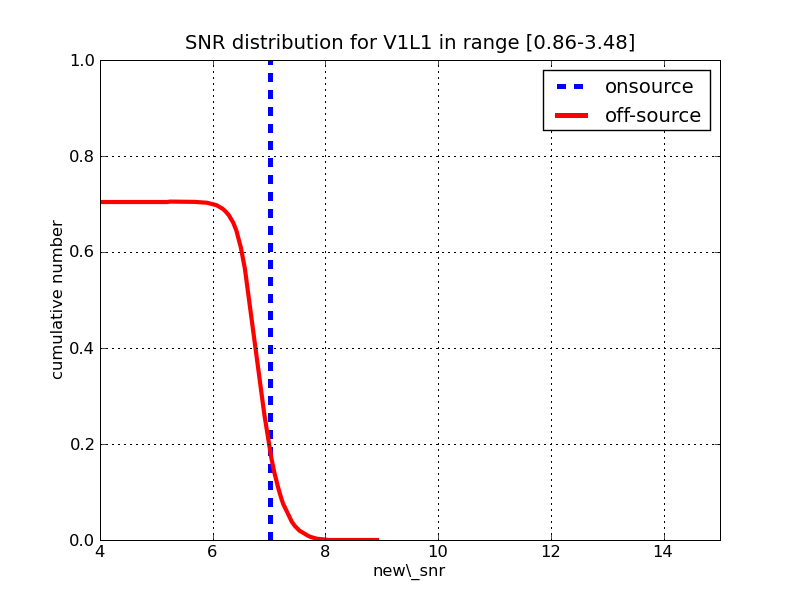
\includegraphics[scale=0.40]{Images/090809B_onsource_slides.png}
%\label{090809B_onsource_slides}
\end{minipage}
\caption{Background distribution (continuous line) and loudest on--source event (dashed line): left figure when no timeslides are performed (``zero--lag''); right figure when 160 timeslides are performed. The timeslides produce events louder that the ``zero--lag'' loudest events.}
\label{090809B_onsource_slides}
%\end{minipage}
\end{figure}

\subsection{Timeslides in the coherent search}

The work in the coincident pipeline is finished; since we are using the coherent pipeline for GRB analyses, we have started the work to implement timeslides in this pipeline as well. The coherent pipeline splits the time series data in segments 128 s long. Long timeslides are just a reshuffling (renaming) of these segments and are done before the FFT and match filtering stages. One may choose to do as many timeslides as desired, they are circular, but there is no point in doing more timeslides than the total number of segments since they repeat themselves (circularily symmetric). Long timeslides are labeled ``long'' since we shift the whole data by a certain amount and not each segment internally, which would be called short timeslides. Long timeslides have already been implemented in the search codes, but the work on postprocessing, involving data quality veto handling, is still to be completed at the time of this writing.

\section{Restriction on inclination angle for nearly face--on binaries}

It is very important to use results of astrophysical observations in GW searches. This is motivated twofold: first, especially in the case of triggered modelled searches, because we want to characterize our target source as accurately as possible. Astrophysically--motivated priors will improve GW detection chances and allow for accurate recovery of parameters. Second, because by using certain astrophysical priors one may reduce the search parameter space and speed up the analysis. 

One such proposed prior would be to limit the inclination angle $\iota$ in the case of a \ac{GW} search triggered by a short GRB. There are two assumptions that lead to a restriction on inclination angle: the jet opening angle from a short burst is small and the \ac{GW} from a short GRB are emitted along the axis of total angular momentum. The first assumption, as we have seen in Chapter \ref{Chapter Two}, is supported by a number of implicit argumets that assume similarity between other high--energy sources that are collimated (AGN, micro--quasars) and short gamma--ray bursts; also, the GRB energetics can be explained by a jet--like emission. There is only one direct astrophysical observation of the jet break for a short burst -- GRB051221A \cite{Burrows:2006ar}, estimating a half--opening angle of 4--8 degrees, but it is believed, analogous to long soft GRBs, that the emission is collimated for short GRBs as well.

We will present a framework allowing us to implement an astrophysical prior on inclination in the case of the coherent analysis pipeline (see Chapter \ref{Chapter Three} for data analysis theory and Chapter \ref{Chapter Four} for pipeline description).

\subsection{Theoretical considerations}

We will consider two separate cases for a short gamma-ray burst produced by a compact binary merger: the binary orbit is ``face--on'' with respect to the GW detectors' plane, i.e., the inclination angle $\iota$ is close to 0 and the binary orbit is ``face--away'' with respect to the GW detectors' plane, i.e., the inclination angle $\iota$ is close to $\pi$. These approximations will be used in computing the amplitude terms $\mathcal{A}^{\mu}$ (see Chapter \ref{Chapter Three} for definitions of amplitude terms) by Taylor--expanding $\cos \iota$ around 0 and $\pi$ keeping only the first leading order terms. The approximation stands well up to angles of order 40 degrees, see Figure \ref{cos_and_approximant}; this is a good indicator that we are not restricting the inclination (and consequently the jet--opening angle) in a too strict of a manner, given that the astrophysical data is not conclusive in the case of short hard GRBs.

\begin{figure}[ht!]
\centering
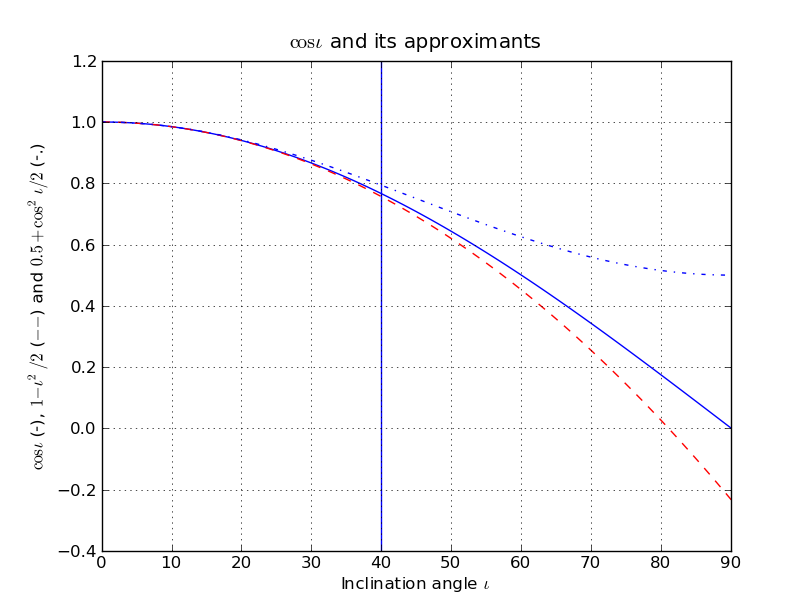
\includegraphics[scale=0.55]{Images/cos_and_approximant.png}
\caption{$\cos \iota$ (continous line) its second--order approximation $1- \frac {{\iota}^2}{2}$ obtained by Taylor--expanding it around 0 (dashed line) and $\frac {1+\cos^2 \iota}{2}$ (dash--dot line). The function and its approximants are almost identical up to high values ($\approx$40 degrees). The same behavior can be seen by Taylor--expanding $\cos \iota$ around $\pi$, with a sign reversion.}
\label{cos_and_approximant}
\end{figure}

\subsubsection{Approximate case $\iota \rightarrow 0$}

Taylor expansion of $\cos \iota$ around 0:
%
\begin{equation}
\cos \iota (\iota \rightarrow 0) = 1- \frac {{\iota}^2}{2}+\frac {{\iota}^4}{4!}+\mathcal{O}({\iota}) \approx 1- \frac {{\iota}^2}{2}
\end{equation}
%
With this in mind we obtain an approximate expression for $\frac {1+\cos^2 \iota}{2}$, expanding again $\cos \iota$ in power series:
%
\begin{equation}
\frac {1+\cos^2 \iota}{2} \approx \frac{1+(1- \iota^2/2! + \iota^4/4!)^2}{2} \approx 1- \frac {{\iota}^2}{2} + \frac {{\iota}^4}{24}\approx 1- \frac {{\iota}^2}{2} \approx \cos \iota,~\iota \rightarrow 0 
\end{equation}
%
We will follow the derivation steps presented in detail in \cite{Harry:2010fr} and summarized in Chapter \ref{Chapter Three}. The waveform amplitudes $\mathcal{A}^{\mu}$, using the expansion of $\cos \iota$, will reduce to:
%
\begin{equation}
\label{eqn:a1}
\mathcal{A}^1 \approx - \frac{D_0}{D} \cos \iota \cos(2(\phi_0-\psi))= - \frac{D_0}{\tilde{D}} \cos (2 \chi_-)
\end{equation}
\begin{equation}
\label{eqn:a2}
\mathcal{A}^2 \approx \frac{D_0}{D} \cos \iota \sin(2(\phi_0-\psi))= \frac{D_0}{\tilde{D}} \sin (2 \chi_-)
\end{equation}
\begin{equation}
\label{eqn:a3}
\mathcal{A}^3 \approx - \frac{D_0}{D} \cos \iota \sin(2(\phi_0-\psi))= - \frac{D_0}{\tilde{D}} \sin (2 \chi_-)
\end{equation}
\begin{equation}
\label{eqn:a4}
\mathcal{A}^4 \approx - \frac{D_0}{D} \cos \iota \cos(2(\phi_0-\psi))= - \frac{D_0}{\tilde{D}} \cos (2 \chi_-)
\end{equation}
%
where $\tilde{D} = D/\cos \iota$ is an effective distance and $\chi_- = \phi_0-\psi$ is an effective phase angle. Therefore, the amplitudes are now function of only two variables, $\tilde{D}$ and $\chi_-$.

Introducing the antenna factors $\mathrm{F}_+=\mathrm{F}_+(\theta, \varphi)$ and $\mathrm{F}_{\times}=\mathrm{F}_{\times}(\theta, \varphi)$ we write the waveform at the detector as $\mathrm{h(t)}= \mathrm{F}_+(\theta, \varphi)\mathrm{h_+(t)}+\mathrm{F}_{\times}(\theta, \varphi)\mathrm{h_{\times}(t)}$ and replacing the amplitude expressions ~(\ref{eqn:a1},~\ref{eqn:a2},~\ref{eqn:a3},~\ref{eqn:a4}) in equation (\ref{eq:h_plus_cross}) we obtain the waveform as a linear combination of the orthogonal complex components $h_0(t)$ and $h_{\pi/2}(t)$. The two polarizations of the gravitational waveform will then be:
%
\begin{eqnarray}
h_+(t) = -\frac{D_0}{\tilde{D}} \cos(2\chi_-) h_0(t) -\frac{D_0}{\tilde{D}} \sin(2\chi_-) h_{\pi/2}(t) \nonumber \\
h_{\times}(t) = \frac{D_0}{\tilde{D}} \sin(2\chi_-) h_0(t) -\frac{D_0}{\tilde{D}} \cos(2\chi_-) h_{\pi/2}(t)
\end{eqnarray}
%
This way the waveforms will depend on only two amplitudes $B_1$ and $B_2$, as opposed to having the four amplitudes from equation (\ref{eq:amplitude_def}):
% 
\begin{eqnarray}
B_1=\frac{D_0}{\tilde{D}}\cos(2\chi_-)=-A^1=-A^4 \nonumber \\
B_2=\frac{D_0}{\tilde{D}}\sin(2\chi_-)=A^2=-A^3
\end{eqnarray}
%
With these, we can express the two gravitational waveform polarizations as
%
\begin{eqnarray}
h_+=-B_1h_0-B_2h_{\pi/2} \nonumber \\
h_{\times}=B_2h_0-B_1h_{\pi/2}
\end{eqnarray}
%
Since CBC signals will spend a large number of cycles in the sensitive band of the detector, the 0 and $\pi/2$ phases will be close to orthogonal, i.e., $(h_0|h_{\pi/2}) \approx 0$ and $(h_0|h_0) \approx (h_{\pi/2}|h_{\pi/2}) = \sigma^2$. We can write the multi--detector log--likelihood expressed by equation (\ref{eq:multi_log_lambda}):
%
\begin{eqnarray}
\mathrm{ln}\Lambda &=& ({\bf s}|{\bf h})- \frac{1}{2}({\bf h}|{\bf h}) \nonumber \\
                   &=& A^{\mu}({\bf s}|h_{\mu}) - \frac{1}{2}A^{\mu}M_{\mu \nu}A^{\nu}
\end{eqnarray}
%
where, $h_{\mu} = (h_1,h_2,h_3,h_4) = (F_+h_0,F_{\times}h_0,F_+h_{\pi/2},F_{\times}h_{\pi/2})$ and, if working in the dominant polarization approximation, $M_{\mu \nu}$ is a diagonal matrix expressed as $M_{\mu \nu}=\mathrm{diag}(\sigma^2F_+^2, \sigma^2F_{\times}^2, \sigma^2F_+^2, \sigma^2F_{\times}^2)$. We will assume summation over the $k$ detectors, but we will write the explicit sum terms only for the final expression, for ease of notation. We wish to express the multi--detector likelihood as function of $B_1$ and $B_2$ only:
%
\begin{eqnarray}
\mathrm{ln}\Lambda &=&-B_1\left((s|F_+h_0)+(s|F_{\times}h_{\pi/2})\right)+B_2\left((s|F_{\times}h_0)-(s|F_+h_{\pi/2})\right) \nonumber \\
        &&-\frac{1}{2}\left(B^2_1+B^2_2\right)(\sigma^2F_+^2+\sigma^2F_{\times}^2)
\label{liken}
\end{eqnarray}
%
Maximizing the likelihood $\Lambda$ function over the two amplitude parameters $B_1$ and $B_2$, gives us the amplitudes values:
%
\begin{eqnarray}
B_1=\frac{(s|F_+h_0)+(s|F_{\times}h_{\pi/2})}{\sigma^2F_+^2+\sigma^2F_{\times}^2}~~\mathrm{and} \nonumber \\
B_2=-\frac{(s|F_{\times}h_0)-(s|F_+h_{\pi/2})}{\sigma^2F_+^2+\sigma^2F_{\times}^2}
\end{eqnarray}
%
and replacing these expressions in the likelihood (\ref{liken}) and introducing summation over the $k$ number of detectors:
%
\begin{eqnarray}
\rho^2&:=&2\mathrm{ln}\Lambda|_{\mathrm{max}} \nonumber \\ 
       &=& \frac{\left(\sum_k(s^k|F_+^kh_0^k)+\sum_k(s^k|F_{\times}^kh_{\pi/2}^k)\right)^2+\left(\sum_k(s^k|F_{\times}^kh_0^k)-\sum_k(s^k|F_+^kh_{\pi/2}^k)\right)^2}{\sum_k\left(F_+^{k,2}+F_{\times}^{k,2}\right)(h_0^k|h_0^k)} \nonumber \\
       &&
\end{eqnarray}
%
it is easy to see that the SNR is now $\chi^2$ distributed with two degrees of freedom.

\subsubsection{Approximate case $\iota \rightarrow \pi$}
Following the same steps as above, Taylor--expanding $\cos \iota$ around $\pi$ this time and replacing in the new values:
%
\begin{equation}
\cos \iota (\iota \rightarrow \pi) = -1+ \frac {{\iota}^2}{2}+\mathcal{O}({\iota}^4) \approx -1+ \frac {{\iota}^2}{2}
\end{equation}
%
and 
%
\begin{equation}
\frac {1+\cos^2 \iota}{2} \approx -\cos \iota,\iota \rightarrow \pi 
\end{equation}
In this case, as above, the expressions for the approximate amplitudes will be:
%
\begin{equation}
\label{eqn:a12}
A_1 \approx - \frac{D_0}{D} \cos \iota \cos(2(\phi_0+\Psi))= - \frac{D_0}{\tilde{D}} \cos (2 \chi_+)
\end{equation}
\begin{equation}
\label{eqn:a22}
A_2 \approx \frac{D_0}{D} \cos \iota \sin(2(\phi_0+\Psi))= \frac{D_0}{\tilde{D}} \sin (2 \chi_+)
\end{equation}
\begin{equation}
\label{eqn:a32}
A_3 \approx - \frac{D_0}{D} \cos \iota \sin(2(\phi_0+\Psi))= - \frac{D_0}{\tilde{D}} \sin (2 \chi_+)
\end{equation}
\begin{equation}
\label{eqn:a42}
A_4 \approx - \frac{D_0}{D} \cos \iota \cos(2(\phi_0+\Psi))= - \frac{D_0}{\tilde{D}} \cos (2 \chi_+)
\end{equation}
%
where, again, $\tilde{D} = D/\cos \iota$ is an effective distance and $\chi_+ = \phi_0+\psi$ is an effective phase angle. Therefore, the amplitudes are again function of only two variables, $\tilde{D}$ and $\chi_+$. In a similar manner, the two GW polarizations are:
%
\begin{eqnarray}
h_+(t) = \frac{D_0}{\tilde{D}} \cos(2\chi_+) h_0(t) +\frac{D_0}{\tilde{D}} \sin(2\chi_+) h_{\pi/2}(t) \nonumber \\
h_{\times}(t) = \frac{D_0}{\tilde{D}} \sin(2\chi_+) h_0(t) -\frac{D_0}{\tilde{D}} \cos(2\chi_+) h_{\pi/2}(t)
\end{eqnarray}

Using the same reduced amplitude terms $B_1$ and $B_2$, the polarizations simplify to
%
\begin{eqnarray}
h_+=B_1h_0+B_2h_{\pi/2} \nonumber \\
h_{\times}=B_2h_0-B_1h_{\pi/2}
\end{eqnarray}
%
We will use the same derivation steps for the multi--detector likelihood as in the case $\iota \rightarrow 0$, maximizing over the amplitude terms$B_1$ and $B_2$, and replacing the amplitude expressions in the likelihood, we obtain:
%
\begin{eqnarray}
\rho^2&:=&2\mathrm{ln}\Lambda|_{\mathrm{max}} \nonumber \\ 
       &=& \frac{\left(\sum_k(s^k|F_+^kh_0^k)-\sum_k(s^k|F_{\times}^kh_{\pi/2}^k)\right)^2+\left(\sum_k(s^k|F_{\times}^kh_0^k)+\sum_k(s^k|F_+^kh_{\pi/2}^k)\right)^2}{\sum_k\left(F_+^{k,2}+F_{\times}^{k,2}\right)(h_0^k|h_0^k)} \nonumber \\
       &&
\end{eqnarray}
%
it is easy to see that the SNR is again $\chi^2$ distributed with two degrees of freedom.

The new detection statistic will be distributed as two $\chi^2$ distributions with 2 degrees of freedom each, each for the $\iota \rightarrow 0$ and $\iota \rightarrow \pi$ cases. We wish to compare this statistic to the standard coherent SNR that is $\chi^2$--distributed with 4 degrees of freedom, given by equation (\ref{eq:fstat_plus_cross}) (see Chapter \ref{Chapter Three}). The difference between two $\chi^2$ distributions with 2 degrees of freedom each and one with 4 degrees of freedom can be seen in Figure \ref{chi_2_and_4}. We notice a decrease of FAP at fixed SNR of roughly one order of magnitude and an increase in sensitivity at fixed FAP of roughly 5\%. The increase in sensitivity could be larger in real noise since glitches tend to give high SNR in only one detector, hence best matched by an edge--on case; this could prove efficient as a glitch--rejection mechanism.

\begin{figure}[ht!]
\centering
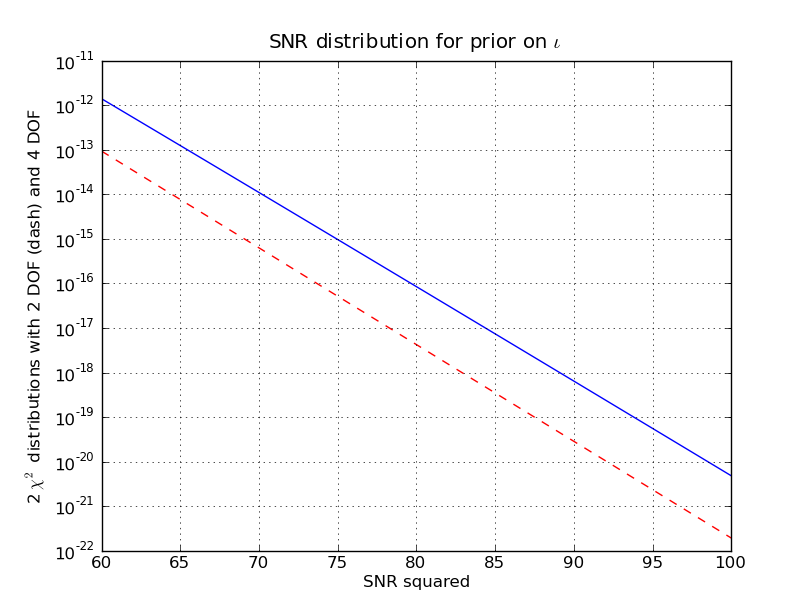
\includegraphics[scale=0.60]{Images/chi_sq_2_and_4.png}
\caption{Difference between two $\chi^2$ distributions with 2 degrees of freedom (DOF) each (dashed red line) and one with 4 DOF (blue continuous line) -- semilog--$y$; the $\rho^2$ represents the network SNR. Imposing a $\iota \rightarrow 0$ or $\iota \rightarrow \pi$ condition in the analysis, generates an SNR that is two $\chi^2$ ,2 DOF each, distributed, whereas the standard coherent SNR is $\chi^2$ ,4 DOF, distributed. We notice a decrease of FAP at fixed SNR of roughly one order of magnitude and an increase in sensitivity at fixed FAP of roughly 5\%.}
\label{chi_2_and_4}
\end{figure}

\section{Discussion}

In this chapter we have introduced a number of developments to the existing templated triggered searches associated with short GRBs. We have estimated, in a very naive way, the probability of a GRB to occur within the detection range of the present LIGO and Virgo. This probability should be comparable to the false alarm probability of any given ``on--source'' event in order for us to attempt at a detection claim. The very low value of this astrophysically motivated probability prompted us to investigate methods that lead to a better estimation of the GW background. We have introduced and presented the theoretical framework and implementation of a method that estimates the background for a coincident triggered GW--GRB search using timeslides. This method uses unphysical time segments that are produced by time--sliding physical data segments from different GW detectors. The main advantage of such a method is that it reduces the error of the background false alarm rate; this method proves most efficient in the case of data from GW detectors with low and similar trigger rates. The implementation of timeslides in the CBC code is relatively straightforward and uses much of the already present infrastructure; the main challenge in implementing it was handling the data quality vetoes.

Based on the assumption that short GRB are highly beamed, we have presented the theoretical framework for a method that restricts the binary inclination angle $\iota$ to 0 or $\pi$, when performing a GW--GRB analysis. This method is still to be tested and implemented, but the theoretical predictions show an increase in search sensitivity of $\sim$5\% at a fixed FAP or a decrease in FAP of one order of magnitude at fixed SNR, compared to a search that draws $\iota$ values uniformly between 0 and $\pi$. This would prove to be a strong ``glitch''--rejection mechanism as well, given that non--Gaussian triggers will have recovered inclination angles randomly distributed between 0 and $\pi$. In terms of errors, a variation $\delta \iota \ll \iota$ would introduce an error term of order $\iota \delta \iota \ll 1$ to first order approximation. The implementation of this restrictive method will be using a relatively large window for the inclination angle, so that to account for wider--jet scenarios, but small enough for the approximations to hold. 

